\documentclass[12pt,a4paper]{report}

\usepackage[left=1.25in,right=1in,top=1in,bottom=1in]{geometry}
\usepackage{tgtermes} % Times New Roman metric equivalent (TeX Gyre Termes)
\usepackage{setspace}
\onehalfspacing
\usepackage{titlesec}
\usepackage{graphicx}
\usepackage{float}
\usepackage{booktabs}
\usepackage{caption}
\usepackage{tikz}
\usetikzlibrary{arrows.meta,positioning}
\usepackage{fancyhdr}
\usepackage[hidelinks]{hyperref}

\setlength{\parskip}{0.4em}
\setlength{\parindent}{1.25em}

\captionsetup{font=normalsize,labelfont=bf,skip=6pt}

\titleformat{\chapter}[display]
  {\normalfont\fontsize{16}{22}\selectfont\bfseries\centering}
  {\MakeUppercase{\chaptertitlename\ \thechapter}}
  {0.45em}
  {\MakeUppercase}
\titlespacing*{\chapter}{0pt}{0pt}{14pt}

\titleformat{\section}
  {\normalfont\fontsize{14}{18}\selectfont\bfseries}
  {\thesection}
  {0.6em}
  {}
\titlespacing*{\section}{0pt}{12pt}{6pt}

\titleformat{\subsection}
  {\normalfont\fontsize{12}{16}\selectfont\bfseries}
  {\thesubsection}
  {0.6em}
  {}
\titlespacing*{\subsection}{0pt}{10pt}{4pt}

\pagestyle{fancy}
\fancyhf{}
\fancyfoot[C]{\thepage}
\renewcommand{\headrulewidth}{0pt}
\renewcommand{\footrulewidth}{0pt}
\fancypagestyle{plain}{%
  \fancyhf{}%
  \fancyfoot[C]{\thepage}%
  \renewcommand{\headrulewidth}{0pt}%
}

\begin{document}

%---------------- Title page ----------------
\begin{titlepage}
\hypersetup{pageanchor=false}
\thispagestyle{empty}
\centering
\vspace*{0.15in}

\includegraphics[width=0.78\textwidth]{uu-logo.png}\\[0.35in]
{\fontsize{16}{22}\selectfont\bfseries FINAL YEAR PROJECT REPORT}\\[0.12in]
{\fontsize{12}{16}\selectfont Phase-2}\\[0.28in]
{\fontsize{16}{22}\selectfont\bfseries SMART BUS MANAGEMENT SYSTEM\\ FOR BANGLADESH}\\[0.18in]
{\normalsize A web platform for route search, seat booking, QR tickets, and fleet control}\\[0.38in]

{\fontsize{14}{18}\selectfont\bfseries PRESENTED BY}\\[0.16in]
\begin{tabular}{@{}ll@{}}
Niropum Sarker Nirjon & ID: 2231081003 \\
Mehrab Hossain & ID: 2231081017 \\
Ahanaf Nafim & ID: 2231081131 \\
\end{tabular}\\[0.08in]
B.Sc.\ in Computer Science and Engineering\\[0.28in]

{\fontsize{14}{18}\selectfont\bfseries SUPERVISED BY}\\[0.14in]
Riasaad Haque Aneek\\
Senior Lecturer, Department of CSE\\[0.32in]

Department of Computer Science and Engineering\\
Uttara University\\[0.18in]
Thesis Defense \textperiodcentered\ October 2026
\end{titlepage}
\hypersetup{pageanchor=true}

%---------------- Abstract ----------------
\chapter*{ABSTRACT}
\addcontentsline{toc}{chapter}{ABSTRACT}
This report presents a bus management system for intercity travel in Bangladesh. Passengers still buy many tickets at counters, while operators keep buses, drivers, and schedules in separate tools. The project joins those tasks in one role-based web application. A passenger searches a route and date, selects a seat, and receives a ticket with a QR code. An administrator manages companies, buses, routes, schedules, and drivers. A driver sees assigned trips. Ticket staff can check a ticket by serial number or QR code.

The system is built with Next.js, TypeScript, Prisma, and PostgreSQL on Supabase, and it is deployed on Vercel. The live database, observed on 11 October 2026, holds 20 bus companies, 200 buses, 848 active routes, 62 drivers, and 7,859 schedules. Seven bookings and a recorded revenue of BDT 3,170 show that the booking path works, but daily use is still small. The main operational limit is the trip calendar: if trip dates are not refreshed, search returns no buses even when the route catalog is large. Future work is a daily trip refresh, one real mobile-payment gateway, and GPS positions sent from the bus.

\vspace{0.6em}
\noindent\textbf{Keywords:} bus management, seat booking, QR ticket, fleet operations, Bangladesh, web application

\tableofcontents
\listoffigures
\listoftables

%---------------- Chapter 1 ----------------
\chapter{INTRODUCTION}
\label{ch:intro}

\section{Introduction}
Road transport carries most intercity passengers in Bangladesh. A traveler who wants a seat on a coach from Dhaka to Chattogram, Sylhet, or Cox's Bazar often depends on a counter, a phone call, or a website that belongs to only one operator. The operator, in turn, may track buses, drivers, and departures in notebooks or in software that passengers never see. The result is a gap between the ticket the passenger holds and the fleet the company runs.

This project designs and deploys one web system for that gap. The public side supports route search, seat selection, and an electronic ticket. The private side supports companies, buses, routes, schedules, drivers, bookings, and ticket checks. Four roles share the same database: passenger, driver, company or platform staff, and super administrator.

\section{Background}
Bangladesh has eight divisions and 64 districts. Intercity coaches connect the main terminals in these districts. Large operators already sell some seats online, but a student, a small operator, and a platform administrator do not share one record of the seat. A sold seat can still appear free at another counter. A driver may not see the same trip list that the office printed in the morning. An administrator who wants occupancy or revenue must collect numbers from several places.

Mobile financial services are already familiar to passengers. That habit does not, by itself, fix seat inventory. A payment succeeds only if the seat record, the trip date, and the ticket can be checked later at boarding. This project therefore treats booking, ticket identity, and fleet records as one problem, not as three separate websites.

\section{Problem Statement}
The problem addressed in this project is the absence of a shared system that links passenger booking with operator fleet control. Existing counters and separate websites do not share seats, trips, and tickets. Passengers cannot rely on one search across operators. Operators cannot see the same trip the passenger just booked. Staff at the gate cannot always verify that a ticket belongs to a real seat on that date.

\section{Objectives}
The project has four objectives:
\begin{enumerate}
  \item Build one platform for passengers, operators, drivers, and administrators.
  \item Digitize route search, seat selection, and QR tickets.
  \item Store buses, schedules, drivers, and companies in one database.
  \item Deploy the system and report what the live deployment actually contains.
\end{enumerate}

\section{Scope}
The system covers intercity bus operations in Bangladesh. In scope are user registration and login, company records, buses and seats, routes and stops, schedules, trip dates, passenger search, seat booking, a ticket with a QR code, ticket verification, driver trip lists, and an operations dashboard. Maintenance, parcels, lost-and-found, and an emergency alert screen are present as supporting modules.

Out of scope for this phase are a live connection to bKash, Nagad, or a card gateway, and GPS hardware on the bus. The interface can name those payment methods, but money movement through a bank or mobile wallet is not completed. Map screens do not yet receive a continuous position from the vehicle.

\section{Significance}
The work matters for three groups. Passengers get one place to search a route and choose a seat. Operators get one record of buses, drivers, and departures instead of separate files. Examiners and future developers get a deployed system whose numbers can be checked, including its limits. The contribution is not a new fare formula. It is a working, role-based operations platform for Bangladesh bus routes, with an honest account of what the live data shows.

%---------------- Chapter 2 ----------------
\chapter{LITERATURE REVIEW}
\label{ch:lit}

\section{Literature Review}
Online ticket systems are a common software project. Ghara et al.\ describe a web portal for bus ticket reservation, cancellation, and route enquiry, aimed at removing long queues at counters \cite{ghara2022}. Their system is a single booking site. It does not separate a platform administrator from many bus companies, and it does not define a QR check at boarding.

Fitriani and Abdillah report an Android application so that passengers can book a seat, see a departure list, and avoid waiting only at an outlet \cite{fitriani2017}. The contribution is mobile access. An operator dashboard, driver assignment, and a shared seat inventory across companies are outside that work.

Digital payment in Bangladesh is studied separately from bus operations. Das examines how university students adopt digital payment and how they judge speed and ease of use \cite{das2024}. Azam studies electronic-commerce adoption by individuals in Bangladesh \cite{azam2023}. Both papers explain why passengers will accept an online step. Neither paper connects a payment record to a seat on a scheduled trip.

\section{Existing Methods}
Three methods are in use today.

\textbf{Counter booking.} A clerk sells a paper seat. The method needs little software. It fails when two counters sell the same seat, and it leaves no shared history for the driver or for a later audit.

\textbf{Single-operator websites.} One company publishes its own coaches. Search and payment can be good for that company. A passenger who does not yet know the company must repeat the search. A platform administrator cannot see every operator in one list.

\textbf{Isolated office tools.} Some operators keep buses and drivers in spreadsheets or in software that passengers cannot open. The ticket and the fleet record diverge as soon as a trip is delayed or a bus is replaced.

Table~\ref{tab:methods} compares these methods with the proposed system on three points that a defense panel can check: whether seat search is online, how many roles the software serves, and whether a ticket can be verified by QR code.

\begin{table}[ht]
\centering
\caption{Comparison of booking methods}
\label{tab:methods}
\renewcommand{\arraystretch}{1.25}
\setlength{\arrayrulewidth}{0.6pt}
\begin{tabular}{|l|l|l|l|}
\hline
\textbf{Method} & \textbf{Seat search} & \textbf{User roles} & \textbf{QR ticket} \\
\hline
Counter booking & Manual & One desk & Paper slip \\
\hline
Single-operator site & Online & Passenger & Often partial \\
\hline
This system & Online & Four roles & Yes \\
\hline
\end{tabular}
\end{table}

\section{Research Gap}
Prior systems show that a queue can be replaced by a website or a phone application \cite{ghara2022,fitriani2017}. Payment studies show that people in Bangladesh already use digital channels \cite{das2024,azam2023}. The gap is the missing link between those two facts and daily fleet control. A useful system must answer, in one database, which company owns the bus, which driver is assigned, which seats are free on a given date, and which ticket code proves the sale. This project targets that gap. It does not claim a new machine-learning model or a completed national payment switch.

%---------------- Chapter 3 ----------------
\chapter{METHODOLOGY}
\label{ch:method}

\section{Methodology and System Workflow}
The work follows a build-and-evaluate path rather than a laboratory experiment. Requirements came from the roles that already exist in a bus company: the passenger, the driver, the operator, and the platform administrator. Each role received only the screens that match that job. Data about districts, routes, and operators were loaded into PostgreSQL. The application was deployed, and the live dashboard was read on 11 October 2026.

Figure~\ref{fig:flow} shows the passenger path. Search does not invent buses in the browser. The server loads trips for the requested route and date, then returns only seats that are still free.

\begin{figure}[ht]
\centering
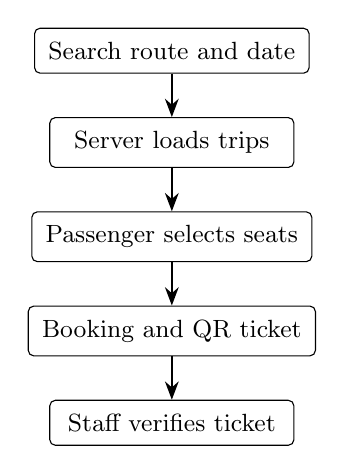
\begin{tikzpicture}[
  node distance=0.55cm,
  box/.style={draw, rounded corners=2pt, align=center, inner sep=5pt, font=\small, minimum width=3.1cm}
]
\node[box] (a) {Search route and date};
\node[box, below=of a] (b) {Server loads trips};
\node[box, below=of b] (c) {Passenger selects seats};
\node[box, below=of c] (d) {Booking and QR ticket};
\node[box, below=of d] (e) {Staff verifies ticket};
\draw[-{Stealth}, thick] (a) -- (b);
\draw[-{Stealth}, thick] (b) -- (c);
\draw[-{Stealth}, thick] (c) -- (d);
\draw[-{Stealth}, thick] (d) -- (e);
\end{tikzpicture}
\caption{Passenger booking workflow}
\label{fig:flow}
\end{figure}

Figure~\ref{fig:arch} is the system architecture. The browser never writes to the database. Pages for passengers, administrators, and drivers call Next.js server actions. Those actions apply the booking and role rules, then read and write PostgreSQL on Supabase.

\begin{figure}[H]
\centering
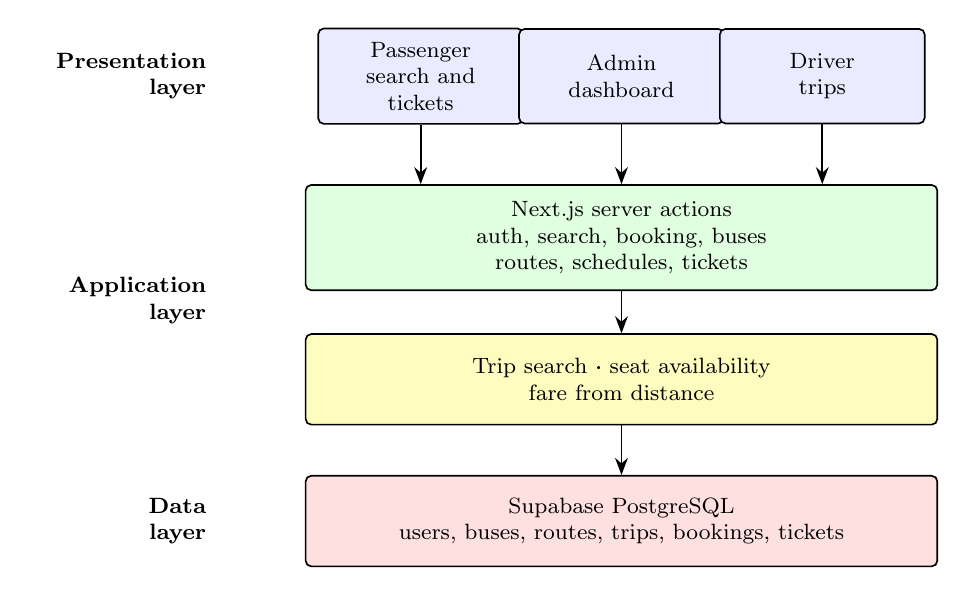
\begin{tikzpicture}[
  >=Stealth,
  ui/.style={
    draw, line width=0.6pt, rounded corners=2pt, fill=blue!8,
    align=center, text width=2.25cm, inner sep=5pt,
    minimum height=1.2cm, font=\footnotesize, anchor=center
  },
  band/.style={
    draw, line width=0.6pt, rounded corners=2pt,
    align=center, text width=7.6cm, inner sep=6pt,
    minimum height=1.15cm, font=\footnotesize, anchor=center
  },
  title/.style={font=\footnotesize\bfseries, align=right, anchor=east, text width=2.15cm}
]
\node[title] at (-5.15, 0) {Presentation\\layer};
\node[ui] (ui1) at (-2.55, 0) {Passenger\\search and tickets};
\node[ui] (ui2) at (0, 0) {Admin\\dashboard};
\node[ui] (ui3) at (2.55, 0) {Driver\\trips};

\node[title] at (-5.15, -2.85) {Application\\layer};
\node[band, fill=green!12] (act) at (0, -2.05)
  {Next.js server actions\\auth, search, booking, buses\\routes, schedules, tickets};
\node[band, fill=yellow!25] (svc) at (0, -3.85)
  {Trip search \textperiodcentered\ seat availability\\fare from distance};

\node[title] at (-5.15, -5.65) {Data\\layer};
\node[band, fill=red!12] (db) at (0, -5.65)
  {Supabase PostgreSQL\\users, buses, routes, trips, bookings, tickets};

\draw[-{Stealth}, line width=0.7pt] (ui1.south) -- (ui1.south |- act.north);
\draw[-{Stealth}, line width=0.7pt] (ui2.south) -- (act.north);
\draw[-{Stealth}, line width=0.7pt] (ui3.south) -- (ui3.south |- act.north);
\draw[-{Stealth}, line width=0.7pt] (act.south) -- (svc.north);
\draw[-{Stealth}, line width=0.7pt] (svc.south) -- (db.north);
\end{tikzpicture}
\caption{System architecture: interface, server actions, and database}
\label{fig:arch}
\end{figure}

The same database serves the other roles. An administrator creates or edits routes, buses, drivers, and schedules. A schedule is a repeating plan: bus, driver, departure time, and days of the week. A trip is that plan on one calendar date. Booking attaches a passenger to a seat on a trip. The ticket stores a number that staff can type or scan. This split between schedule and trip is the main design decision. It allows one weekly plan to produce many dated departures without copying the route each morning by hand.

\section{Data, Algorithms, and Tools}
\subsection{Data}
Route and place data cover the geography the interface must search: divisions, districts, upazilas, terminals, and intercity routes. Each route stores source, destination, and distance. Fare is derived from distance at a fixed rate of 3 BDT per kilometre when a stored fare is missing, so a route without a manual price still has a defined charge. Buses have a seat grid. Companies, drivers, and users are separate records linked by role.

The live deployment, read from the operations dashboard on 11 October 2026, contained the counts in Table~\ref{tab:live}. These figures are operational counts, not accuracy scores. The project is a software system, so the evaluation does not report precision or F1.

\begin{table}[ht]
\centering
\caption{Live deployment counts on 11 October 2026}
\label{tab:live}
\renewcommand{\arraystretch}{1.25}
\setlength{\arrayrulewidth}{0.6pt}
\begin{tabular}{|l|r|}
\hline
\textbf{Item} & \textbf{Count} \\
\hline
Bus companies (active) & 20 \\
\hline
Buses & 200 \\
\hline
Active routes & 848 \\
\hline
Drivers & 62 \\
\hline
Schedules & 7{,}859 \\
\hline
Terminals & 41 \\
\hline
Bookings (all dates) & 7 \\
\hline
Bookings on that day & 0 \\
\hline
Recorded revenue & BDT 3{,}170 \\
\hline
\end{tabular}
\end{table}

\subsection{Algorithms and Tools}
There is no trained model. The core procedure is a search over trips. Given a source, a destination, and a date, the server selects active trips on that date whose route matches, hides departed trips when the date is today, and returns free seats. Seat choice is a direct map: a seat is free if no confirmed or pending booking holds it. The important rule sits on the server, so the browser cannot mark a sold seat as free.

The implementation stack is TypeScript and Next.js~16 on Vercel, Prisma as the database client, and PostgreSQL hosted on Supabase. Authentication uses Better Auth with email and password and role checks before a dashboard opens. The public site and the admin site are the same application, separated by role after login. Source code is maintained at the project repository, and the running site is the Vercel deployment used for the counts above \cite{nextjs2026,prisma2026}.

\section{Evaluation and Expected Outcomes}
\subsection{Evaluation}
Evaluation checks whether the deployed system meets the four objectives, using the live site rather than a local demo only.

The platform objective is met. Login separates a super administrator from other roles, and the dashboard lists companies, buses, routes, drivers, bookings, payments, and ticket verification. The digitizing objective is met in the interface: a passenger can search, open a seat map, and receive a ticket that staff can verify by code or QR scan. The database objective is met: one PostgreSQL schema holds the records, with row-level security enabled so the anonymous public key is not a second administration path. The reporting objective is met by Table~\ref{tab:live}, with two limits stated below.

A search for Dhaka to Chattogram on 11 October 2026 returned no buses. The dashboard showed zero trips for that calendar day, while a much larger set of older trip rows still existed. The route catalog was not empty. The dated trips had not been rolled forward to the defense week. Occupancy on that day was 0\%, and daily revenue was BDT 0, which matches the empty search. Seven historical bookings and BDT 3,170 show that the booking tables are used, not that the system is busy every day.

\subsection{Expected Outcomes}
If trip dates are generated for today and the next seven days on every active schedule, popular routes should show a bookable list without adding hundreds of unused buses to every route. A practical target is about 7 to 20 coaches on a busy route for that week. One payment gateway, starting with bKash or Nagad in sandbox mode, should replace the current claim that several wallets are already connected. A later study can attach a phone or tracker on the bus and store positions against the trip, which the present map screen does not do.

The outcome of this phase is a deployed role-based bus system for Bangladesh, with measured coverage and a clear list of what is not finished. That is a stronger result than a slide that reports an accuracy percentage the software never computed.

%---------------- References ----------------
\begin{thebibliography}{9}
\bibitem{ghara2022}
S.~Ghara, T.~Saha, A.~Ghosh, D.~Biswas, and A.~Das, ``Online quick bus ticket reservation system,'' \emph{Int.\ J.\ Res.\ Appl.\ Sci.\ Eng.\ Technol.}, vol.~10, no.~5, pp.~4409--4414, May 2022, doi: 10.22214/ijraset.2022.43408.

\bibitem{fitriani2017}
Fitriani and L.~A. Abdillah, ``Android-based bus ticket reservation application,'' OSF Preprints, 2017, doi: 10.31227/osf.io/5a7eb.

\bibitem{das2024}
A.~C.~Das, ``Understanding the dynamics of digital payment adoption among public university students of Bangladesh,'' Research Square, preprint, 2024, doi: 10.21203/rs.3.rs-4138836/v1.

\bibitem{azam2023}
M.~S.~Azam, ``Adoption of electronic commerce by individuals in Bangladesh,'' \emph{Inf.\ Develop.}, vol.~39, no.~4, 2023, doi: 10.1177/02666669211052523.

\bibitem{nextjs2026}
Vercel, ``Next.js documentation,'' 2026. [Online]. Available: \url{https://nextjs.org/docs}

\bibitem{prisma2026}
Prisma, ``Prisma ORM documentation,'' 2026. [Online]. Available: \url{https://www.prisma.io/docs}

\end{thebibliography}

\end{document}
